\section{Nao Software}
Um Nao auf einfache Weise zu programmieren, simulieren oder ihm neue Funktionen beizubringen gibt es im wesentlichen zwei Programme. Diese werden im folgenden jeweils kurz vorgestellt:
\\
\\
\noindent
\textbf{Choregraphe} 
\\
Choregraphe ist eine multi - plattform Desktopanwendung. Mit ihrer Hilfe ist es möglich:
\begin{itemize}
\item Neue Animationen und Verhalten zu erstellen,
\item diese entweder auf einem simulierten  oder direkt auf einem realen Roboter zu testen und
\item den Roboter dabei zu überwachen und zu steuern.
\end{itemize}
Dabei steht die Einfachheit der Anwendung im Vordergrund und so ist es auch möglich sehr komplexe Verhalten (z.B. Interaktion mit Menschen, Tanzen oder E-Mails verschicken) zu implementieren ohne eine einzige Zeile Quellcode selbst zu schreiben. Zusätzlich ist die Möglichkeit gegeben, vorhandenen Code mit eigenem Python - Code zu erweitern.

\begin{figure}[H]						
	\centering							
	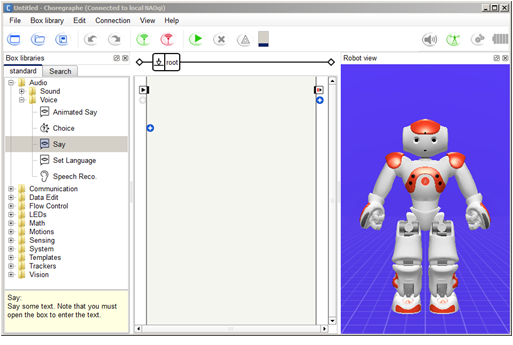
\includegraphics[scale=1.0]{Bilder/choregraphe.png}			
	\caption{Überblick Choregraphe}						
	\label{f:nao_choregraphe}						
\end{figure}

Abbildung \ref{f:nao_choregraphe} zeigt einen Überblick über alle Subfenster und Panels innerhalb Choregraphe. Wie zu sehen, ist Choregraphe zentral in drei Bereiche unterteilt: Links, Mitte und Rechts.
Auf der linken Seite ist die sogenannte Box - Bibliothek zu finden. Dort sind alle von Haus aus gespeicherten Bewegungen und Verhalten abrufbar. Diese können per Drag\&Drop in die Mitte gezogen werden. Die Mitte stellt sozusagen ein Fluss - Diagramm der einzelnen Boxen dar. So ist es möglich \textit{graphisch} zu programmieren (Verknüpfen der Boxen). Auf der rechten Seite ist das Abbild eines Nao - Roboters zu sehen. Dies zeigt, je nach dem, einen simulierten Roboter oder die Spiegelung eines realen Naos. 
Durch diese graphisch einfache Programmierung können auch unerfahrene Anwender mit Nao arbeiten. So ist Nao nicht nur für die Forschung oder für Entwickler gedacht, sondern auch für den Unterricht an Schulen.

Die Programmierung des Roboters geschieht durch Verbinden von einzelnen Boxen. Es ist auch möglich ein Programm mit verschiedenen Wegen zu entwerfen oder Konditionalstrukturen (\textit{if-else-elseif}) einzubauen. Abbildung \ref{f:nao_choregrapheProg} zeigt ein Programm, in welchem der Roboter zu einer gewissen Position laufen soll. Währenddessen überprüft er mittels des Ultraschallsensors, ob ein Hindernis im Weg ist. Bei positivem Ergebnis soll sich der Roboter hinsetzen.

\begin{figure}[H]						
	\centering							
	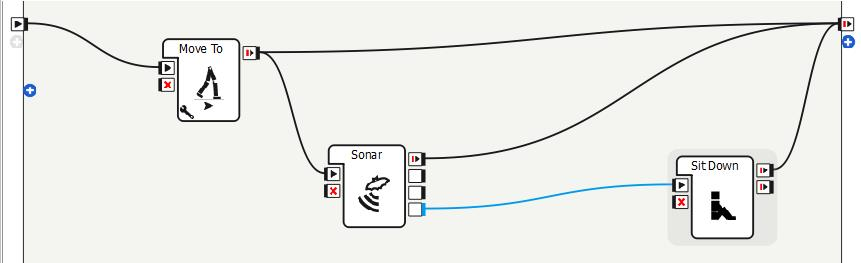
\includegraphics[scale=.6]{Bilder/choregraphe_prog.jpg}			
	\caption{Choregraphe Programmierung}						
	\label{f:nao_choregrapheProg}						
\end{figure}

Neue Bewegungen oder Verhalten können entweder durch eigenen Python - Code oder durch vormachen integriert werden. Dazu kann über eine \textit{Timeline} aufgenommen werden, zu welchem Zeitpunkt der Bewegung sich die einzelnen Gelenke/Körperteile befinden sollen. Anschließend kann diese aufgenommene Timeline als Verhalten in einer Box gespeichert werden.
\\
\\
Die Möglichkeit neue Programme erst an einer Simulation zu testen, spart erstens Akkulaufzeit eines realen Nao und zweitens schützt es diesen vor \textit{schlechten} Programmen, bei denen er Schaden nehmen könnte. Ein weiterer Vorteil ist, dass zu jeder Box der Quellcode in Python sichtbar ist und sich dadurch Arbeit erspart werden kann.
\\
\\
Choregraphe wurde in dieser Arbeit hauptsächlich dazu genutzt, sich in die Marterie Nao einzuarbeiten, seine Funktionsweise zu verstehen und zu erlernen wie er programmiert wird.
\\
\\
\textbf{Webots for Nao}
\\
Webots für Nao erlaubt es, einen simulierten Roboter in einer virtuellen Welt zu bewegen. Die Software bietet eine sichere Umgebung um neue Verhalten zu testen, bevor sie in die reale Welt übertragen werden. Webots for Nao ist eine spezifische Auskopplung von Webots 7, einer professionellen Software zum simulieren diverser Roboter, beispielsweise KUKA - Robotern oder Lego Mindstorms. Mit Webots for Nao können jedoch keine anderen Roboter genutzt oder neue erstellt werden.

\begin{figure}[H]						
	\centering							
	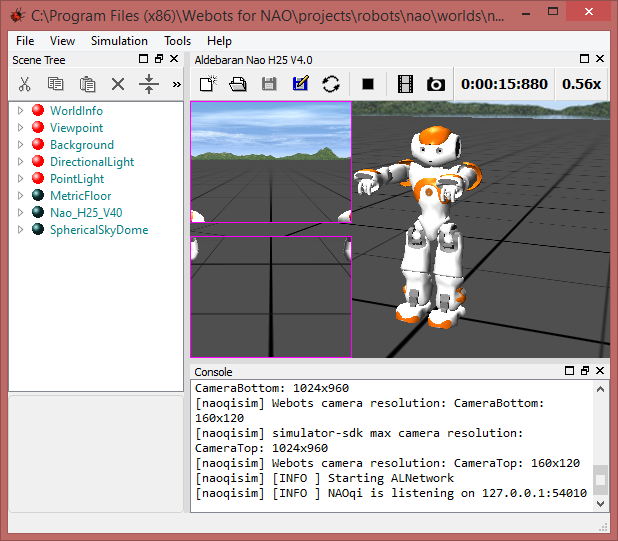
\includegraphics[scale=1.0]{Bilder/webots.png}			
	\caption{Überblick Webots}						
	\label{f:nao_webots}						
\end{figure}
\noindent
Bild \myref{f:nao_webots} zeigt einen simulierten Nao in einer virtuellen Welt. Auf der linken Seite befinden sich Reiter, die ausgeklappt werden können. Dort können Objekte in die Welt gelegt werden. Auf der rechten Seite ist Nao von Vorne und jeweils ein Ausschnitt der beiden Kameras an seinem Kopf zu sehen. Unterhalb davon ist eine Konsole, die verschiedene Angaben ausgibt, z.B. die IP - Adresse und der Port, unter dem der simulierte Nao angesprochen werden kann.

Der Unterschied zu der Simulation in Choregraphe liegt darin, dass in Webots auch Elemente wie Tische, Stühle oder andere Hindernisse in die Welt gelegt werden können. So kann beispielsweise getestet werden, ob Nao Hindernissen ausweicht, wenn er auf sie zu läuft.
\\
\\
Webots wurde im Allgemeinen dafür genutzt, zu Testen, ob die Übertragung der Armwinkel korrekt ist und ob diese der Bewegung durch dem Menschen entsprechen. Würden die Tests an einem realen Nao durchgeführt werden, würden seine Aktoren sehr schnell warm werden und eventuell Schaden davon nehmen.





